\begin{figure}[htb]
\begin{subfigure}[t]{0.35\textwidth}
    \centering
      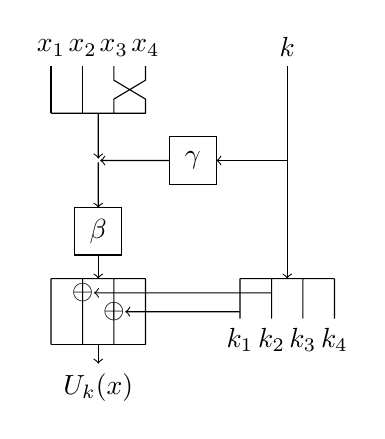
\begin{tikzpicture}[xscale=-0.6, yscale=-0.6]
        % Input bits
        \draw
        (-3.00, 2.80) node(k3){$k_{4}$} 
        (-2.33, 2.80) node(k2){$k_{3}$} 
        (-1.67, 2.80) node(k1){$k_{2}$} 
        (-1.00, 2.80) node(k0){$k_{1}$} 
        (-3.00, 1.50) -- (k3)
        (-2.33, 1.50) -- (k2)
        (-1.67, 1.50) -- (k1)
        (-1.00, 1.50) -- (k0)
        (-3.00, 1.50) -- (-1.00, 1.50);
        \draw
        (+1.00, 3.1) node(x3){}
        (+1.67, 3.1) node(x2){}
        (+2.33, 3.1) node(x1){}
        (+3.00, 3.1) node(x0){} ;
% 		node[not gate US, draw, scale=0.35, rotate=90](not1) at (1.0,2.6) {}
% 		node[not gate US, draw, scale=0.35, rotate=90](not2) at (1.67,2.6) {}
		\draw
        (+1.00, 1.50) -- (x3)
        (+1.67, 1.50) -- (x2)
        (+2.33, 1.50) -- (x1)
        (+3.00, 1.50) -- (x0)
        (+3.00, 1.50) -- (+1.00, 1.50) ;
	
		\draw (+1.0,2.9) -- (+2.0,2.9);
		\draw (+3.0,2.9) -- (+2.0,2.9);
		\draw[->] (+2.0,2.9) -- (+2.0,3.3) node[below=0] {$U_k(x)$};

        % t_in
        \draw
        (-1.00, 2.20) coordinate(k1) (+1.67, 2.20) node[inner sep=0](k1_target){$\oplus$}
        (-1.67, 1.80) coordinate(k0) (+2.33, 1.80) node[inner sep=0](k0_target){$\oplus$};
        \draw[->] (k1) -- (k1_target);
        \draw[->] (k0) -- (k0_target);

        % Mini S-Boxes
        \draw (+1.5, +0.0) rectangle (+2.5, +1.0) node[pos=0.5] {$\beta$} ;
        \draw (-0.5, -1.5) rectangle (+0.5, -0.5) node[pos=0.5] {$\gamma$} ;
        \draw (+2.0, -1.0) node[inner sep=0] (mult) {$\fmult$};
        % 4-bits wires
        % left
        \draw[<-] (-2.0, +1.5) -- (-2.0, -1.0) ;
        \draw[->] (-2.0, -1.0) -- (-0.5, -1.0) ;
        \draw     (-2.0, -1.0) -- (-2.0, -3.0) node[above=0.05] {$k$};
        % right
        \draw[<-] (+2.0, +1.5) -- (+2.0, +1.0) ;
        \draw[<-] (+2.0, +0.0) -- (mult);
        \draw[->] (+0.5, -1.0) -- (mult);
        \draw[<-] (mult) -- (+2.0, -2.0);
        % Output bits
        \draw
        (+3.00, -2.00) -- (+1.00, -2.00)
        (+1.00, -2.00) -- (1,-2.3) -- (1.67, -2.7) -- (+1.67, -3.0) node[above=0.05] {$x_3$}
        (+1.67, -2.00) -- (1.67,-2.3) -- (1, -2.7) -- (+1, -3.0) node[above=0.05] {$x_4$};
%        (+2.33, -2.00) -- (+2.33, -2.3) -- (+3.00, -2.7) -- (+3.00, -3.0) node[above=0.05] {$x_3$}
%        (+3.00, -2.00) -- (+3.00, -2.3) -- (+2.33, -2.7) -- (+2.33, -3.0) node[above=0.05] {$x_4$};

\draw        (+2.33, -2.00) -- (+2.33, -3.0) node[above=0.05] {$x_2$};
\draw        (+3.00, -2.00) -- (+3.00, -3.0) node[above=0.05] {$x_1$};

      \end{tikzpicture}
\end{subfigure}
    %\FigDef{final-u}{Final decomposition of $U_k(x)$.}
\begin{subfigure}[t]{0.58\textwidth}
    \vspace{-5cm} % hack...
    \centering
      \renewcommand\arraystretch{1.3}
      \setlength{\tabcolsep}{2pt}
      \footnotesize
      \centering
      \begin{tabular}{l|rrrrrrrrrrrrrrrr}
 ~&~ $\hex{0}$ & $\hex{1}$ & $\hex{2}$ & $\hex{3}$ & $\hex{4}$ & $\hex{5}$ & $\hex{6}$ & $\hex{7}$ & $\hex{8}$ & $\hex{9}$ & $\hex{a}$ & $\hex{b}$ & $\hex{c}$ & $\hex{d}$ & $\hex{e}$ & $\hex{f}$\\
        \hline
$\alpha$ ~&~ $\hex{c}$ & $\hex{c}$ & $\hex{c}$ & $\hex{c}$ & $\hex{8}$ & $\hex{8}$ & $\hex{8}$ & $\hex{8}$ & $\hex{e}$ & $\hex{e}$ & $\hex{e}$ & $\hex{e}$ & $\hex{a}$ & $\hex{a}$ & $\hex{a}$ & $\hex{a}$\\
$\beta$ ~&~ $\hex{0}$ & $\hex{e}$ & $\hex{b}$ & $\hex{4}$ & $\hex{2}$ & $\hex{3}$ & $\hex{f}$ & $\hex{8}$ & $\hex{a}$ & $\hex{7}$ & $\hex{1}$ & $\hex{9}$ & $\hex{5}$ & $\hex{c}$ & $\hex{6}$ & $\hex{d}$\\
$\gamma$ ~&~ $\hex{1}$ & $\hex{d}$ & $\hex{1}$ & $\hex{6}$ & $\hex{5}$ & $\hex{3}$ & $\hex{a}$ & $\hex{5}$ & $\hex{e}$ & $\hex{7}$ & $\hex{9}$ & $\hex{6}$ & $\hex{8}$ & $\hex{7}$ & $\hex{e}$ & $\hex{1}$\\
$\swaplsb$ ~&~ $\hex{0}$ & $\hex{2}$ & $\hex{1}$ & $\hex{3}$ & $\hex{4}$ & $\hex{6}$ & $\hex{5}$ & $\hex{7}$ & $\hex{8}$ & $\hex{a}$ & $\hex{9}$ & $\hex{b}$ & $\hex{c}$ & $\hex{e}$ & $\hex{d}$ & $\hex{f}$\\
      \end{tabular}
    %   \vspace{1cm}
    %   }{
    %   \TabDef{u-books}{Functions $\alpha,\beta,\gamma,\swaplsb$.}
    %   }
%   \end{floatrow}
\end{subfigure}
\FigDef{final-u}{The decomposition of $U_k(x)$.}
\end{figure}